\chapter{Informationsteoretiske Nedre Grænser og Modstander Nedre Grænser for sortering ved sammenligninger}

\section{En $\Omega (n \log n)$ nedre grænse til sortering ved sammenligninger}%
\label{sec:sorteringsalgoritmesammenligninger}

\begin{note}[Kilder]
Video 24 \\
\href{https://imada.sdu.dk/u/jbj/DM553/LBnoteJBJ21.pdf}{Kapitel 7 - Jørgens noter til nedre grænser}
\end{note}

Vores mål her er at vise at en modstander altid vil kunne tvinge $\frac{1}{2}n \log n$ sammenligninger i enhver sammenligningsbaseret sorteringsalgoritme. Vi antager at listen der skal sorteres har størrelse $n$, og at $n = 2^{k}$, for et ikke-negativt heltal $k$.Modstanderen har, til at lave sin strategi, et binært træ $T$ af dybde $k = \log n$, hvis knuder indeholder elementer. Til at starte med er det kun roden i træet, hvis størrelse ikke er 0, den indeholder nemlig de $n$ elementer der skal sorteres.

Vi giver træet ``niveauer'', sålede at niveau 0 indeholder roden, og niveau $\ell$ indeholder $2^{\ell}$ ``poser''.\footnote{Poser er en anden måde at sige knuder på, vi bruger poser til at betyde knuder der kan indeholde elementer.} Et deltræ $T[b]$ er et deltræ hvor roden er knuden $b$. Ethvert deltræ $T[b]$ på niveau $\ell$ har den invariant, at størrelsen $|T[b]| \le 2^{k-\ell} = \frac{n}{2^{\ell}}$.\footnote{Invariant betyder at udsagnet som følger holder igennem hele algoritmen.}

I algoritmen som modstanderen bruger når vedkommende svarer på en sammenligning, bevæger hvert element sig ned igennem træet, indtil alle $n$ elementer er i deres egen private pose, af størrelse $1$ på niveau $k-1$.\footnote{$k-1$ fordi roden er niveau $0$ og dybden er $k$.} Når dette sker, er alle elementerne sorteret.

Vi definerer tre tilstande, som en pose $b$ kan være i igennem køringen af algoritmen:
\begin{itemize}
  \item \textbf{Åben}: Både venstre og højre deltræ af $b$  har mindre end $2^{k-\ell-1}$ elementer.
  \item \textbf{Højre-flushed}: Venstre deltræ har størrelse $2^{k-\ell-1}$.
  \item \textbf{Venstre-flushed}: Højre deltræ har størrelse $2^{k-\ell-1}$.\footnote{Jørgens noter har nogle fejl i, som han ikke forklarer i videoen. Jeg har valgt at sige at ``venstre-flush'', betyder at elementerne kan komme ned til venstre deltræ. Derudover forklarer han slet ikke i noterne hvad hhv. right og left-flush er, han antager bare at man ved det.}
\end{itemize}

I Figur~\ref{fig:flushes} ses de tre tilstande for en pose $b$.

\begin{figure}[ht]
\centering
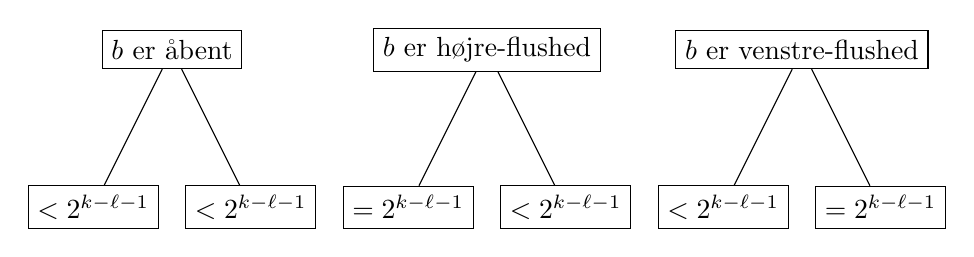
\begin{tikzpicture}[level distance=2cm, sibling distance=2.5cm, every node/.style = {shape=rectangle, draw, align=center}]
% Open state
\node at (-4,0) {$b$ er åbent} [sibling distance=2.0cm]
child {node {$<2^{k-\ell-1}$}}
child {node {$<2^{k-\ell-1}$}};

% Left-flushed state
\node at (0,0) {$b$ er højre-flushed} [sibling distance=2.0cm]
child {node {$=2^{k-\ell-1}$}}
child {node {$<2^{k-\ell-1}$}};

% Right-flushed state
\node at (4,0) {$b$ er venstre-flushed} [sibling distance=2.0cm]
child {node {$<2^{k-\ell-1}$}}
child {node {$=2^{k-\ell-1}$}};
\end{tikzpicture}
  \caption{\label{fig:flushes} De 3 tilstande $b$ kan være i.}
\end{figure}

Til at udføre sin strategi, gør modstanderen brug af følgende funktioner:
\begin{itemize}
  \item \textbf{MOVE(u)}: Denne funktion kaldes når et element $u$ er kommet til posen $b'$, og gør som følger:
        \begin{itemize}
          \item Hvis $b'$ er \textbf{åbent} forbliver $u$ i $b'$.
          \item Hvis $b'$ er \textbf{højre-flushed} eller \textbf{venstre-flushed} bliver elementet $u$ flyttet til posen $b'$ på hhv. højre eller venstre deltræ. Derefter bliver \textbf{MOVE(u)} kaldt igen.
        \end{itemize}
  \item \textbf{CHECK(u)}: Denne funktion kaldes ved en åben pose $b$, og gør som følger:
        \begin{itemize}
          \item Tjekker om enten højre eller venstre deltræ $T[b]$ af posen $b$ på niveau $\ell$ indeholder $2^{k-\ell-1}$ elementer, og hvis så, markerer den pose $b$ hhv. venstre eller højre-flushed.
          \item Kalder \textbf{MOVE} på \textit{alle} elementer i $b$.
        \end{itemize}
\end{itemize}

I Algoritme~\ref{alg:move} og Algoritme~\ref{alg:check} kan algoritmiske fortolkninger ses af hhv. CHECK og MOVE.

\begin{algorithm}
\caption{\label{alg:move} MOVE(u)}
\begin{algorithmic}[1]
\STATE $b(u)$ \COMMENT{Nuværende pose af $u$}
\IF{$b(u)$ er åben}
    \RETURN
\ELSIF{$b(u)$ er venstre-flushed}
    \STATE $b(u) \gets b^L(u)$
    \STATE MOVE($u$)
    \RETURN
\ELSIF{$b(u)$ er højre-flushed}
    \STATE $b(u) \gets b^R(u)$
    \STATE MOVE($u$)
    \RETURN
\ENDIF
\end{algorithmic}
\end{algorithm}

\begin{algorithm}
\caption{\label{alg:check} CHECK(b)}
\begin{algorithmic}[1]
\STATE $b$ er en åben pose på niveau $\ell$
\IF{$|T[b^R]| = 2^{k-\ell-1}$}
    \STATE Marker $b$ som venstre-flushed \COMMENT{højre undertræ er fyldt}
    \STATE MOVE($u$)
    \RETURN
\ENDIF
\IF{$|T[b^L]| = 2^{k-\ell-1}$}
    \STATE Marker $b$ som højre-flushed \COMMENT{venstre undertræ er fyldt}
    \STATE MOVE($u$)
    \RETURN
\ENDIF
\RETURN
\end{algorithmic}
\end{algorithm}

\subsection{Modstanderens Strategi}%
\label{subsec:label}

Imens modstanderen svarer på spørgsmål om $x < y$ fra algoritmen, så flytter den enten 2, 1, eller 0 elementer ned i træet, men \textbf{en undtagelse}: Efter hvert \textit{MOVE(u)} kald på et element $u$ fra posen $b$, kalder vi \textit{CHECK(b)}, som kan flytte op til $2^{k-\ell -1}$ elementer. Efter hver query som resulterer i at mindst et element flyttes, kaldes \textit{MOVE(u)} rekursivt på elementet.

Antag at sorteringsalgoritmen $A$ efterspørger resultatet på en sammenligning af elementer $u$ og $v$. Lad \(\ell(u)\) og \(\ell(v)\) være niveauene af hhv. $l$ og $v$. Lad $b(u)$ og $b(v)$ være poserne der indeholder henholdvis $u$ og $v$.

\begin{enumerate}
  \item Hvis den mindste fælles forfader (least comon ancestor) $b$ af $b(u)$ og $b(v)$ i $T$ ikke er $b(u)$ eller $b(v)$, så svarer modstanderen ``$u < v$'' hvis $u$ er i det venstre undertræ af $b$ og $v$ i det højre, og ``$v < u$'', hvis $u$ er i det højre undertræ af $b$ og $u$ i det venstre. Intet element flyttes her. $A$ får ingen information ud af den her sammenligning.
  \item Hvis den mindste fælles forfader $b$ af $b(u)$ og $b(v)$ er i $\{b(u), b(v)\}$, så kan man, uden tab af generalitet, sige at $b = b(u)$ eller $b = b(v)$. Vi antager herfra at $b = b(u)$.
\end{enumerate}





%%% Local Variables:
%%% mode: latex
%%% TeX-engine: xetex
%%% TeX-command-extra-options: "-shell-escape"
%%% TeX-master: "main"
%%% End:
